\documentclass{report}
\usepackage{graphicx} % Required for inserting images
\usepackage[italian]{babel}
\usepackage{tikz}
\usepackage{hyperref}
\usepackage{amsmath}
\usepackage{xcolor}
\usepackage{float}
\usepackage{soul}
\usepackage{listings} % Per evidenziare il codice

\definecolor{lightgray}{rgb}{0.9,0.9,0.9} % Definizione colore sfondo
\definecolor{darkgreen}{rgb}{0.0, 0.5, 0.0}

\lstset{
    backgroundcolor=\color{lightgray}, % Sfondo grigio
    basicstyle=\ttfamily, % Font monospaziato
    % frame=single, % Bordo attorno al codice
    tabsize=4, % Dimensione tabulazione
    breaklines=true, % Permette di andare a capo automaticamente
    numbers = left,
    numberstyle=\small\color{gray}
}

\title{\huge\textbf{{Sicurezza dei Sistemi e delle Reti}}}
\date{File di Nali}

\begin{document}

\maketitle

\tableofcontents
\newpage

\chapter{Politiche di Sicurezza}
\section{Definizione Politica di sicurezza}

La \textit{gestione della sicurezza} è un \textit{processo formale} 
per rispondere alle domande:
\begin{itemize}
    \item quali sono i beni da proteggere
    \item quali sono le possibili minacce
    \item come si possono contrastare le minacce 
\end{itemize}

\noindent Questo processo ha natura iterativa, ed è contenuto nella ISO 31000; in 
questa norma viene descritto un \textit{modello per la gestione della sicurezza 
delle informazioni} che comprende le seguenti fasi:
\begin{itemize}
    \item \textbf{Plan:}
    \begin{itemize}
        \item stabilire politiche, processi e procedure di sicurezza
        \item eseguire la valutazione del rischio 
        \item sviluppare un piano di trattamento del rischio 
    \end{itemize}
    \item \textbf{Do:}
    \begin{itemize}
        \item implementare il piano di trattamento del rischio
    \end{itemize}
    \item \textbf{Check:}
    \begin{itemize}
        \item monitorare e mantenere il piano di trattamento del rischio
    \end{itemize}
    \item \textbf{Act:}
    \begin{itemize}
        \item mantenere e migliorare la gestione dei rischi 
        \item risposta ad incidenti, analisi di vulnerabilità e riprendere il ciclo iterativamente
    \end{itemize}
\end{itemize}

\subsection{Definizioni}
\begin{itemize}
    \item \textbf{Rischio:} esprime la possibilità che un attacco causi danni ad una 
    organizzazione
    \item \textbf{Risorsa:} tutto ciò che necessita di essere protetto
    \begin{itemize}
        \item \textit{hw}
        \item \textit{sw}
        \item \textit{reputazione}
    \end{itemize}
    
    \noindent La valutazione di una risorsa viene fatta in base:
    \begin{itemize}
        \item ai costi da sostenere per sostituire la risorsa nel caso non sia più disponibile 
        \item perdita di incassi in caso di attacco 
    \end{itemize}
    \item \textbf{Vulnerabilità:} punti deboli che possono essere sfruttati per causare danni al 
    sistema; possono essere classificate come:
    \begin{itemize}
        \item critico 
        \item moderato 
        \item basso
    \end{itemize}
\end{itemize}

\noindent Definizione per domanda esame: Una politica di sicurezza dei sistemi e delle reti è l'insieme strutturato di regole, requisiti e comportamenti che un'organizzazione definisce affinché i propri sistemi informatici e le proprie infrastrutture di rete applichino in modo coerente misure di protezione contro accessi non autorizzati, abusi, perdite di dati e altri rischi. Essa rappresenta ciò che il sistema deve far rispettare, automatizzando e facendo valere controlli come l'autenticazione, l'autorizzazione, il monitoraggio delle attività e la gestione delle vulnerabilità, allo scopo di garantire la riservatezza, l’integrità e la disponibilità delle informazioni, secondo gli obiettivi stabiliti dall'organizzazione stessa.


\section{Domanda MAC, DAC e RBAC}
\begin{center}
    \textit{definire l'utilizzo delle politiche di sicurezza basate su MAC, DAC e RBAC}
\end{center}
\noindent Gli approcci DAC,MAC e RBAC fanno parte delle politiche di controllo degli accessi e forniscono approcci diversi
a seconda del contesto di applicazione
\subsection{DAC (Discretionary Access Control):}
\noindent Il controllo dell'accesso viene fatto sull' \textbf{identità del soggetto richiedente} e delle \textbf{regole di accesso}.
Definito \textit{discrezionale} poichè un'entità potrebbe avere i privilegi di accessi che le permettono, a sua volta, di concedere l'accesso ad un'altra entità.

\noindent Si può rappresentare mediante una matrice, dove:
\begin{itemize}
    \item le colonne rappresentano i soggetti
    \item le righe gli oggetti
    \item ogni cella specifica i diritti di accesso di quel soggetto a quel determinato oggetto
\end{itemize}


\subsection{MAC (Mandatory Access Control):} 
La politica di controllo degli accesssi MAC, o Mandatory Access Controll si basa sul confronto tra \textbf{etichette di sicurezza} che indicano quanto sono sensibili le risorse
e \textbf{autorizzazioni di sicurezza} che indicano quali entità del sistema sono idonee ad accedere a quali risorse.

\noindent Questa politica è definita \textit{mandatoria} poichè un'entità che possiede l'accesso a una risorsa non può estendere il permesso di acesso a un'altra entità,
può farlo solo l'amministratore di sistema.

\noindent I sistemi MAC si dividono in:
\begin{itemize}
    \item \textbf{Multilevel security systems:} consiste in una struttura verticale di sistemi di sicurezza, agli utent viene assegnato un livello e possono accedere solo a risorse con un livello uguale o inferiore
    \item \textbf{Multilateral security systems:} l'accesso viene assegnato in base a segmenti che formano gruppi costituiti da livelli di sicurezza e parole in codice
    \begin{itemize}
        \item si ottiene una struttura orizzontale, che contiene livelli di sicurezza verticali aggiuntivi
    \end{itemize}
\end{itemize}

\noindent Vantaggi:
\begin{itemize}
    \item molto sicuro, a prova di manomissione
    \item gli utenti non possono fare modifiche
    \item controllo automatizzato
    \item i dati non possono essere modificati senza apposita autorizzazione
\end{itemize}

\noindent Svantaggi:
\begin{itemize}
    \item richiede una pianificazione dettagliata e un lavoro amministrativo
    \item controllo e aggiornamento dei dati di accesso
    \item manutenzione per aggiunta di nuovi dati o utenti e relative modifiche (elevato carico di lavoro per l'amministratore)
\end{itemize}

\subsection{RBAC (Role Based Access Control):}
\noindent Introduce il concetto di \textbf{ruolo}, ovvero una funzione che può essere assiciata a uno o più utenti (gli utenti possono avere più ruoli)
e una \textbf{sessione}, ovvero una mappatura tra utente e un sottoinsieme di ruoli a cui è assegnato.

\noindent I ruoli di un utente possono fornire o meno accesso a determinate risorse.

\noindent Quattro tipi di entità:
\begin{itemize}
    \item \textbf{Utente:} una persona che ha accesso al sistema, ogni individuo ha un ID associato
    \item \textbf{Ruolo:} funzione lavorativa all'interno dell'organizzazione
    \item \textbf{Autorizzazione:} approvazione di una modalità di accesso ad uno o più oggetti
    \item \textbf{Sessione:} mappatura tra utente e un sottoinsieme dei ruoli a cui è assegnato
\end{itemize}

\section{Fare cenni sull'utilizzo di tali politiche nei Sistemi Operativi moderni}
\subsection{Unix security model}
In Linux ci sono tre entità da considerare:
\begin{itemize}
    \item \textbf{Soggetto:} può essere un utente o un processo 
    \item \textbf{Oggetto:} file, cartelle, \dots
    \item \textbf{Operazioni consentite:} lettura, scrittura, esecuzione 
\end{itemize}

\noindent In Unix, ogni utente ha associato un id univoco, detto \textbf{UID}; può appartenere a 
gruppi di utenti, anch'essi identificati da un id univoco detto \textbf{GID}. Tutti gli utenti 
appartenenti ad un gruppo possono condividere tra loro oggetti.

\noindent Ad ogni file è assegnato un unico utente proprietario e un unico gruppo proprietario. L'autorizzazione 
viene concessa mediante una ACL che identifica le operazioni che i soggetti possono fare.

\subsubsection{Processi in Linux}
Ogni processo è isolato dagli altri e non possono accedere alla memoria altrui. Ogni processo viene 
eseguito con le autorizzazione dell'UID dell'utente che lo sta eseguendo. 

\noindent Nel momento della creazione, ad ogni processo sono assegnati tre ID (inizialmente tutti uguali 
all'UID):
\begin{itemize}
    \item \textbf{Effective UID:} determina le autorizzazioni per il processo 
    \item \textbf{Real UID:} determina l'utente che ha avviato il processo 
    \item \textbf{Saved UID:} EUID prima di eventuali modifiche
\end{itemize}

\noindent L'utente \textit{root} può cambiare EUID/RUID/SUID a valori arbitrari; utenti non privilegiati
possono cambiare EUID solo a RUID o SUID

\subsubsection{Unix file access control}
Le modifiche agli ID sono apportate mediante i comandi \textit{setUID} e \textit{setGID}; questa modifica 
permette ai programmi non privilegiati di accedere a risorse generalmente non accessibili.

\noindent Le directory possono aver impostato uno \textit{\textbf{sticky bit}}: specifica che solo il proprietario di un file nella cartella
può apportare una modifica a quel file 

\noindent Il \textit{\textbf{superuser}} è esente dalle consuete restrizioni di controllo degli accessi, ha 
accesso a tutto il sistema.


\subsection{Windows security architecture}
L'architettura di sicurezza di Windows è basata su più entità:
\begin{itemize}
    \item \textbf{\textit{Security Reference Model (SRM):}} componente che in modalità kernel esegue 
    controlli delle autorizzazioni e manipola i privilegi degli utenti
    \item \textbf{\textit{Local Security Authority (LSA):}} risiede in un processo utente, è responsabile 
    dell'applicazione della politica di sicurezza locale, tra cui:
    \begin{itemize}
        \item criteri per le password, come complessità e tempi di scadenza 
        \item politica di controllo $\rightarrow$ specifica quali operazioni su quali oggetti vadano controllate 
        \item impostazioni dei privilegi
    \end{itemize}
    \item \textbf{\textit{Security Account Manager (SAM):}} è un database che archivia i dati degli account e le 
    informazioni di sicurezza su entità locali e gruppi
    \item \textbf{\textit{Active Directory (AD):}} implementa il protocollo LDAP (\textit{Lightweight Directory Access Protocol})
\end{itemize}

\subsubsection{Windows security model}
Windows ha un complesso sistema di controllo dell'accesso; ogni oggetto ha ACL per permettere autorizzazioni 
granulari ad utenti e/o gruppi di utenti.

\subsubsection{Security descriptor}
Ogni oggetto ha un \textit{security descriptor} che contiene:
\begin{itemize}
    \item \textbf{\textit{security identifier} (SID)} per il possessore e il gruppo primario dell'oggetto (SID è 
    associato univocamente ad ogni utente) 
    \item \textbf{\textit{discretionary ACL} (DACL):} diritti di accesso per gli utenti e i gruppi
    \item \textbf{\textit{system ACL} (SACL):} tipi di accesso che generano log
\end{itemize}

\noindent Ad ogni processo viene inoltre associato un insieme di \textbf{token}, che prende il nome di 
\textbf{\textit{security context}}. Nel momento in cui un processo vuole accedere ad un oggetto, presenta 
il suo insieme di token e il sistema controlla se il security context abbia o meno accesso a tale risorsa 
in base al \textit{security descriptor} dell'oggetto.



\chapter{Set-UID}
\section{Si definisca il funzionamento e possibili implicazioni per la sicurezza}
Il meccanismo SETUID in Unix/Linux consente a un programma di essere eseguito con i privilegi dell’utente proprietario del file, anziché con quelli dell’utente che lo esegue. È spesso usato per permettere a utenti comuni di svolgere operazioni che richiedono privilegi elevati, come accedere a risorse di sistema. Tuttavia, questa funzionalità ha implicazioni di sicurezza importanti: se un programma con SETUID è vulnerabile o mal scritto, può essere sfruttato per ottenere privilegi superiori, fino a diventare root. Per questo motivo, l’uso di SETUID è considerato delicato e va limitato a programmi essenziali e attentamente controllati.

\subsection{Esempio di utilizzo di SETUID}
Un esempio semplice di utilizzo del SetUID è un programma che consente a un utente normale di scrivere in un file accessibile solo a root. Normalmente, un utente senza privilegi non potrebbe modificare file di sistema, ma se il programma è di proprietà di root e ha il bit SetUID attivo, verrà eseguito con i privilegi di root anche se l’utente che lo lancia non li possiede. In questo modo, il programma può svolgere un’operazione riservata, come scrivere in un file protetto, 
senza dover dare all’utente l’accesso diretto a quei privilegi. Questo dimostra come SetUID possa essere usato per concedere temporaneamente diritti elevati in modo controllato.

\section{Ogni processo Unix process è associato con un real user ID (RUID) e un effective user ID (EUID). Spiegare la logica ed importanza del setuid.}
Il \textbf{Real User ID} (RUID) , determina l'utente che ha avviato il processo, mentre l'Effective User ID (EUID), determina le autorizzazioni per il processo.
Il \textbf{set user ID} (setuid) ha due funzioni principali: permette a un utente di eseguire un file o un processo con i privilegi dell'utente proprietario, oltre che ai suoi. Inoltre consente a programmi privilegiati di accedere a risorse generalmente non accessibili.
Questo può comportare problematiche su sistemi, se impostato in maniera non corretta, oltre che essere una vulnerabilità che può essere sfruttata per attacchi.
\subsection{Quale tra RUID e EUID viene utilizzato dal sistema operativo per determinare se un processo
ha il diritto di accedere a una risorsa o meno?}
Il sistema operativo verifica il EUID per determinare se un processo ha diritto ad accedere a una risorsa o meno.
\subsection{Nella maggior parte delle versioni di Unix, la famiglia di funzioni setuid consente di impostare l'EUID di un processo sul suo RUID. Riesci a pensare a un motivo per farlo in un processo in esecuzione come root (EUID=0)?}
Quando si deve andare a modificare la password di un utente, si deve andare a modificare un file chiamato shadow: questo file è modificabile solo dall'utente root, perciò lanciando il comando passwd, il processo setta come ID quello di root, per permettere la modifica di questo file.




\section{Esercizi con codice}


\subsection{Charlie ha trovato nel computer un file con i seguenti permessi:}
\noindent \textbf{-rwsrwxrwx 1 root root 186 Oct 31 23:42 mioexe}

\noindent \textbf{Spiegare la pericolosità del file mioexe.}

\noindent Il file mioexe ha tutti i permessi settati, quindi sia l'owner, che il gruppo a cui appartiene, che tutti gli altri utenti, possono leggere, scrivere ed eseguire il file.
Inoltre è impostato il SUID, un permesso speciale che indica al kernel di lanciare i comandi con i privilegi dell'owner del file: in questo caso l'owner è root, 
perciò si potrebbe modificare il file mioexe per lanciare dei comandi dannosi come root.

\subsection{Come esempio si consideri /usr/bin/passwd : spiegare se tale comando ha il setuid settato e
perché}
Il comando `/usr/bin/passwd` ha il bit SETUID attivo perché permette a un utente normale di modificare la propria password, operazione che richiede l'accesso al file di sistema `/etc/shadow`, il quale è leggibile e scrivibile solo dall'utente root.

\noindent Grazie al SETUID, quando un utente esegue `passwd`, il processo assume temporaneamente i privilegi di root (proprietario del file), così da poter aggiornare in sicurezza la password nel file protetto. Questo è un classico esempio di uso legittimo e necessario del SETUID, ma proprio per la sua sensibilità, il comando `passwd` deve essere scritto in modo estremamente sicuro per evitare rischi di escalation dei privilegi.

\subsection{Commentare l'esecuzione di passwd dal seguente processo}
\begin{figure}[H]
    \centering
    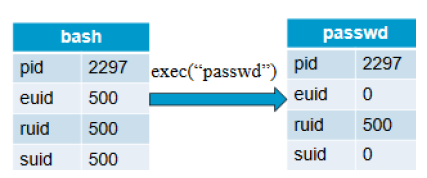
\includegraphics[width=0.8\linewidth]{images/psswd.png}
\end{figure}
Lanciando il comando passwd, si indica al sistema operativo di voler cambiare la propria password utente. Questa password è presente in un file chiamato shadow, che è modificabile solo dall'utente root.
Lanciando quindi il comando passwd, si va a indicare che il EUID è uguale a 0, cioè l'utente root, fornendo temporaneamente all'utente con RUID 500 di modificare la propria password.

\subsection{Si consideri l'utente bob che appartiene solo al gruppo users. Per ognuno dei seguenti file, discutere se bob è capace di eseguire il file, se no spiegare perchè, se sì evidenziare i bit EUID e RUID dei corrispondenti processi.}
\subsubsection{-rwsr--r-- 1 root root 213 Oct 12 11:10 file1.bin}
Si, può eseguire il file perché, anche se potrebbe solo leggerlo, è impostato il setUID (s) e quindi può eseguirlo con i privilegi del owner (cioè di root). RUID è quello di Bob, mentre EUID è 0, cioè quello di root

\subsubsection{-rwxr-xr-- 1 alice users 134 Oct 12 11:11 file2.bin}
Si, può eseguire il file perché fa parte del gruppo del owner del file (alice, che è del gruppo users). Non potrà però scriverci, in quanto non dispone del privilegio (r-x). In questo caso RUID e EUID corrispondono e sono quelli di Bob.

\subsubsection{-rwsr-xr-- 1 alice users 186 Oct 12 11:12 file3.bin}
Si, può eseguire il file perché fa parte del gruppo del owner del file (alice, che è del gruppo users). A differenza di sopra però, è impostato il SETUID, perciò Bob lancia il comando come se fosse Alice. RUID = Bob, EUID = Alice

\subsubsection{-r--rwxr-- 1 bob users 113 Oct 12 11:13 file4.bin}
No, in questo caso l’owner del file è Bob, ma non ha i privilegi per poter eseguire il file. I membri del suo gruppo, users invece possono leggere, scrivere ed eseguirlo, il che è un po’ un controsenso.

\subsection{Si immagini che un attaccante trovi una shell di root su un terminale e digiti le seguenti righe di codice, quali conseguenze potrebbe avere?}
\subsubsection{\% cp $/$ bin$/$sh $/$tmp$/$ break-acct }
\subsubsection{\% chmod 4755 $/$tmp$/$break-acct}
L’attaccante, con il primo comando, copia la shell in una cartella temporanea. Con il secondo comando assegna il bit SetUID (il 4 davanti a 755), in modo che, quando un altro utente esegue quel file, la shell venga avviata con i privilegi del proprietario, cioè root. Questo permette a qualsiasi utente di ottenere una shell come root, con la possibilità di fare gravi danni al sistema.
La parte 755 dei permessi indica che il proprietario può leggere, scrivere ed eseguire il file, mentre gli altri utenti (gruppo e altri) possono leggere ed eseguire (ma non scrivere).

\subsection{Descrivere cosa succede al file readme.txt dopo l’esecuzione dei comandi visualizzati in figura}
\begin{figure}[H]
    \centering
    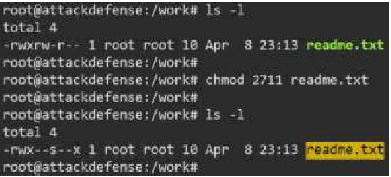
\includegraphics[width=0.8\linewidth]{images/readme.png}
\end{figure}
Il file readme.txt ha subito un comando per modificarne i permessi (chmod) e gli è stato settato il bit “set Group ID” (2), mentre l’owner può leggere, scrivere ed eseguire il file (7). I membri del suo gruppo e tutti gli altri utenti invece possono solo eseguire il file.
Readme.txt diventa quindi un file eseguibile chi lo esegue, lo fa come se fosse nel gruppo del owner, piuttosto che nel suo.

\subsection{Programma catall.c}
\begin{figure}[H]
    \centering
    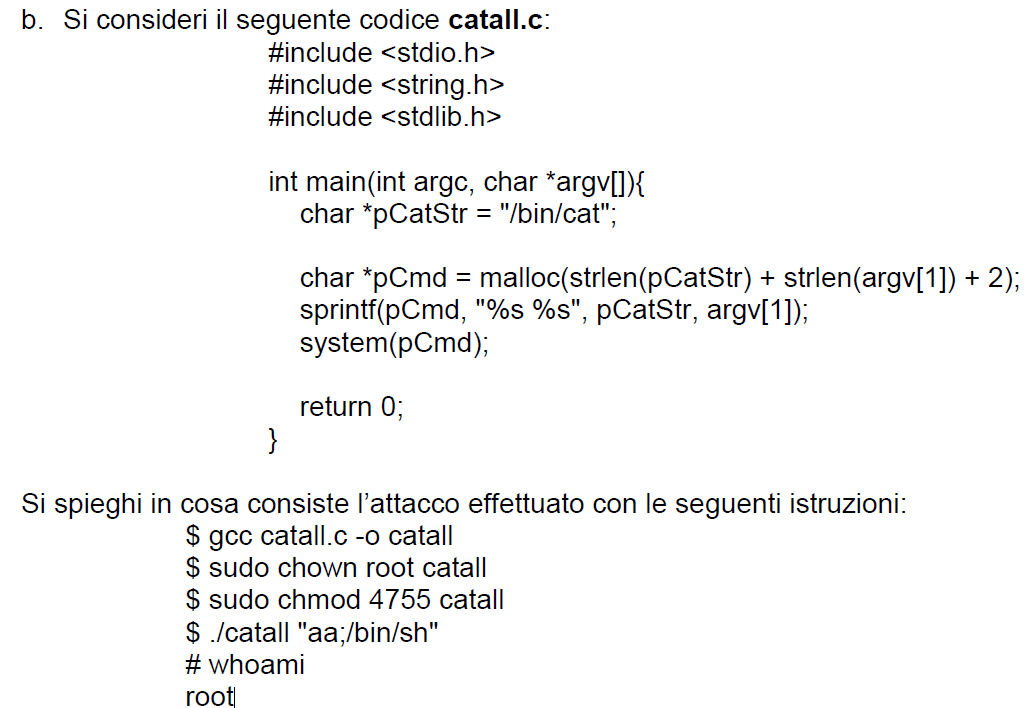
\includegraphics[width=0.8\linewidth]{images/setuidsettembre2024.png}
\end{figure}
In questo caso, il programma `catall` viene compilato e poi configurato con il bit SetUID, rendendolo eseguibile con i privilegi di root. Il programma prende un argomento da linea di comando e lo concatena al comando `/bin/cat`, eseguendolo tramite `system()`. Il problema di sicurezza nasce dal fatto che l’argomento dell’utente viene inserito direttamente in una stringa di comando senza alcun controllo.

Quando '’attaccante lancia `./catall "aa;/bin/sh"`, il programma esegue effettivamente due comandi: prima `cat aa`, poi, a causa del punto e virgola, viene eseguito anche `/bin/sh`. Poiché il programma ha i privilegi di root, anche la shell ottenuta è con privilegi di root. Questo permette all’attaccante di accedere a una shell di amministratore, aggirando le normali restrizioni. L'istruzione `whoami` confermerà infatti che l’utente è root. Questo è un esempio di escalation dei privilegi dovuto a un uso non sicuro della funzione `system()` in un programma SetUID.







\chapter{Malware}
\noindent Una definizione informale per malware potrebbe essere quella di \textit{programma malevolo},
solitamente inserito di nascosto in un sistema, che ha lo scopo di compromettere la \textbf{riservatezza}, l'\textbf{integrità} o la \textbf{disponibilità} 
del sistema stesso.

\noindent I malware sono classificati in base a:
\begin{itemize}
    \item \textbf{Propagazione:} software, rete, social engeneering
    \item \textbf{Azioni sui dati colpiti:} corruzione, furto, crittografia
    \item \textbf{Attack kit:} strumenti già pronti per attaccare
    \item \textbf{Attori e/o motivazioni dell'attacco}
\end{itemize}

\section{Differenza tra due tipologie di malware (virus e worm) + esempio}
\noindent Sono stati chiesti questi due ma per sicurezza aggiungo anche gli altri
\subsection{Trojan}
È un programma che ha un effetto evidente e atteso dall'utente, che ha però anche un 
effetto \textbf{nascosto} che viola le politiche di sicurezza e che viene condotto senza l'autorizzazione 
dell'utente

\subsection{Virus}
È un codice che può replicarsi modificando altri file o programmi per inserire codice in 
grado di replicarsi a sua volta; questa \textbf{proprietà di replicazione} è ciò distingue 
i virus dagli altri tipi di malware. Non svolge nessuna azione evidente, ma cerca di rimanere 
nell'ombra.

\noindent La replica richiede un certo tipo di assistenza da parte dell'utente, come ad esempio
cliccare su un allegato.

\noindent Un virus è composto da tre parti:
\begin{itemize}
    \item \textbf{Meccanismo di infezione}
    \item \textbf{Trigger:} evento che determina quando il payload viene attivato
    \item \textbf{Payload:} cosa fa il virus (oltre a diffondersi)
\end{itemize}

\noindent I virus attraversano quattro fasi:
\begin{enumerate}
    \item \textbf{Dormiente:} il virus è inattivo in attesa di essere attivato 
    \item \textbf{Scatenante:} il virus viene attivato 
    \item \textbf{Propagazione:} il virus inserisce una copia di sé stesso in certe parti del sistema; ogni programma 
    infetto conterrà ora un altro virus che entrerà a sua volta in fase di propagazione 
    \item \textbf{Esecutiva:} la funzione viene eseguita
\end{enumerate}

\subsubsection{Vettori di infezione}
I principali vettori di infezione sono:
\begin{itemize}
    \item \textbf{Boot sector} di dispositivi esterni; il codice è inserito nel boot sector e viene 
    eseguito in fase di avvio 
    \item \textbf{Eseguibili}
    \item \textbf{File macro:} il virus si attacca ai documenti per propagarsi 
\end{itemize}

\subsubsection{Esempio noto in letteratura:}
Un esempio di virus può essere considerato il compression virus, che va a comprimere lo spazio occupato da un programma, per inserire un codice malevolo:
così facendo la dimensione di un file è la stessa, andando a baypassare i controlli di un antivirus.

\subsection{Worm}
I worm sono programmi \textit{stand alone} (a differenza dei virus che devono essere attivati 
da un qualche evento) in grado di replicarsi.

\noindent Le fasi di esecuzione sono:
\begin{itemize}
    \item \textbf{Probing:} cerca informazioni sulla macchina 
    \item \textbf{Expoloitation:} sfrutta le informazioni raccolte per trovare vulnerabilità
    \item \textbf{Replicazione}
    \item \textbf{Attacco} (payload)
\end{itemize}

\subsubsection{Esempio noto in litteratura:}
Esempio di worm della famiglia Nimda, che prese di mira i sistemi operativi Microsoft Windows.

\subsection{Drive-by-download}
Sfruttano \textbf{vulnerabilità del browser} per installare codice malevolo ad insaputa dell'utente 
nel momento in cui visita la pagina web dell'attaccante. 

\subsection{Clickjacking}
L'attaccante intercetta un \textit{click} dell'utente per costringerlo a fare delle cose 
contro la sua volontà.

\subsection{Zombie e botnet}
Lo \textit{zombie} è una singola macchina, mentre la \textit{botnet} è un insieme di macchine 
zombie controllate da una singola entità; vengono usate per fare DDoS, phishing, spamming, \dots

\subsection{Rootkit}
È un insieme di programmi installati su un sistema per mantenere l'accesso ad un sistema, ad 
esempio, con privilegi di amministratore, nascondendo le prove della sua presenza e aggirando 
i meccanismi di controllo.

\noindent Permettono di fare attacchi anche con scarse conoscenze tecniche.

\subsection{Scareware}
Software che hanno lo scopo di diffondere shock, ansia e/o la percezione di una minaccia; sono 
un attacco di \textit{social engeneering}.

\subsection{Ransomware}
Software che tiene in ostaggio il sistema per richiedere un riscatto all'utente, spesso tramite
cifratura.

\subsection{Vulnerabilità zero-day}
Si intende un'exploit non ancora nota e che non ha quindi una contromisura.

\subsection{Spear phishing}
Viene \textbf{studiato nel dettaglio il bersaglio}, in modo tale da fare del phishing più mirato 
ed efficace.

\subsection{Spyware}
Malware che raccoglie piccole informazioni alla volta sugli utenti a loro insaputa,
come ad esempio un \textit{keylogger}.

\subsection{APT - Advanced Persistent Threats}
\begin{itemize}
    \item \textit{\textbf{Advanced:}} è un'applicazione con un ampia varietà di tecnologie di intrusione e malware
    \item \textit{\textbf{Persistent:}}
    attacchi per un periodo di tempo prolungato verso il target
    \item \textit{\textbf{Target:}} target selezionati in modo accurato
\end{itemize}

\noindent Le fasi principali di un attacco tramite APT sono:
\begin{itemize}
    \item \textbf{Ricognizione:} si sceglie una vittima e la si studia 
    \item \textbf{Weaponization:} si mette un trojan che permette accesso remoto in un payload consegnabile (email, USB, web)
    \item \textbf{Sfruttamento:} il codice malevolo viene attivato per portare a termine il suo scopo
\end{itemize}



\section{Differenza tra virus metamorfico e polimorfico}
\subsection{Classificazione dei virus}
È possibile classificare i virus in base alle \textbf{tecniche usate per superare i controlli 
di sistema:}
\begin{itemize}
    \item \textbf{Cifratura del virus:} crea una chiave per \textit{"crittografarsi"}; quando viene 
    chiamato un programma infetto, con tale chiave viene decifrato il virus. Per evitare pattern 
    di bit, durante la propagazione la chiave viene cambiata
    \item \textbf{Stealth virus:} si nasconde dal rilevamento da parte dell'antivirus, tramite mutazione 
    o compressione del codice 
    \item \textbf{Polymorphic virus:} durante la replica crea copie che svolgono la stessa funzione 
    ma che hanno pattern di bit diversi 
    \item \textbf{Metamorphic virus:} si riscrive completamente ad ogni iterazione per aumentare la 
    difficoltà di rilevamento
    \item \textbf{Compression virus:} comprimono il file eseguibile in modo che la versione infetta 
    abbia la stessa dimensione di quella originale
\end{itemize} 

\section{Discutere se le seguenti tecniche sono meccanismi di rilevamento utili rispettivamente per i virus polimorfici e metamorfici:}

\subsection{Static pattern matching}
\noindent Utile per \textbf{virus polimorfici} poichè cambiano solo la parte cifrata del loro codice a ogni infezione, ma mantengono invariata la struttura del decryptor,
che può essere riconosciuto con tecniche di pattern matching statico, perché rimane simile o identico tra le varianti.

\noindent Al contrario dei virus metamorfici che modificano completamente il proprio codice a ogni infezione, incluso il decryptor o qualsiasi parte riconoscibile.

\subsection{Pattern matching during emulation}
\noindent Utile per \textbf{virus metamorfici} poichè nonostante essi cambino completamente aspetto a ogni infezione, 
durante l'emulazione (cioè durante l'esecuzione simulata del codice in un ambiente controllato), il virus esegue le stesse azioni fondamentali, indipendentemente dalla sua forma.

\noindent La tecnica di pattern matching during emulation permette quindi di osservare il comportamento reale del codice eseguito (come accessi a file di sistema, chiamate di sistema sospette, o autoriproduzione).

\noindent Al contrario, emulare un virus polimorfico è inefficiente, perché richiede tempo e risorse per ottenere un'informazione che è già ricavabile staticamente.

\subsection{Suspicious behaviour detection}
\noindent Utile per \textbf{virus polimorfici} poichè il loro comportamento rimane molto prevedibile:
\begin{itemize}
    \item Decriptano il corpo
    \item Si copiano in altri file
    \item Cercano persistenza
\end{itemize}

\noindent Per quanto riguarda i virus metamorfici possono cercare di mascherare il loro comportamento,
soprattutto quelli più avanzati possono simulare comportamenti legittimi.

\noindent Questo li rende più difficili da intercettare solo con behaviour detection




\chapter{Autenticazione}

\section{Discutere le problematiche di autenticazione su Web e in dettaglio uno schema challenge-response}
\noindent L'autenticazione in generale, e in particolare quella web, consiste principalmente in un client che fa una richiesta a un server e un server che fornisce una risposta.

\noindent Per fare in modo però che il server non inivii informazioni a client malevoli, che possono attaccare tramite attacchi di spoofing,
fingendosi un client legittimo (o anche fingendosi un server legittimo), oppure con replay attack, ciò inivio di pacchetti già inviati da un client legittimo(tramite 
sniffing sulla rete), vengono introdotte misure di sicurezza più avanzate.

\noindent Client e server condividono informazioni segrete, che possono andare da una password a una chiave di crittografia(secret):
un client che vuole accedere a un servizio web su un server, deve dimostrare di essere chi dichiara di essere. Il server presenta quindi 
una stringa (\textbf{challenge}) e il client, tramite il secret, può fornire la prova di identificazione richiesta e riesce ad accedere (\textbf{response}).

\noindent Questo schema fornisce segretezza, tramite uso di password o chiavi, e anche freschezza, nella misura in cui la challenge viene modificata a ogni richiesta, così
che non si possa sfruttare una risposta già fornita con un replay attack.


\chapter{Attacchi TCP}

\section{ARP spoofing attack, quali sono le possibili conseguenze ed eventuali contromisure}
\noindent Il protocollo ARP (Address Resolution Protocol) si occupa di connettere un indirizzo fisico (MAC address) con un indirizzo logico(IP address). Per farlo ogni nodo all'interno della rete invia dei messaggi in broadcast
per segnalare la sua presenza, così che gli altri nodi possano andare a popolare e/o modificare una tabella interna chiamata \textit{ARP cache table}

\noindent Viene fatta un'assunzione di trust nella LAN, dato che le richieste non vengono tracciate, gli annunci non sono autenticati, le macchine si fidano l'una dell'altra.
In questo modo un possibile attaccante può utilizzare il meccanismo automatico di aggiornamento della ARP cache table (che si aggiorna anche se non ha inviato alcuna richiesta) per fingersi un altro dispositivo.

\noindent \textbf{Conseguenze:} L'attaccante si impone tra due dispositivi permettendogli di intercettare il traffico (sniffing), modificarlo (per esempio per iniettare un malware) o
bloccarlo (DoS).

\noindent \textbf{Contromisure:} Alcune possibili contromisure possono essere:
\begin{itemize}
    \item ARP statici: si configurano manualmente le associazione degli indirizzi IP e MAC, ma non è pratico in reti dinamiche o di grandi dimensioni
    \item Crittografia del traffico: anche se l'attaccante intercetta il traffico, non può leggerne il contenuto.
    \item Strumenti di monitoraggio 
\end{itemize}

\section{Attacco TCP SYN flood e le sue contromisure + SYN-Cookie}
\noindent L'attacco TCP SYN Flood è una forma di attacco DoS (Denial of Service) che mira a sovraccaricare un server esaurendone le risorse disponibili per le connessioni, impedendo così agli utenti legittimi di accedere ai servizi.
L'idea è di sfruttare le vulnerabilità legate alla negoziazione di una comunicazione tra client e server durante il three-way handshake, l'attaccante \textbf{continua a iniviare richieste SYN al server} senza poi rispondere ai SYN/ACK ricevuti in risposta,
il server dovrà quindi attendere andando a saturare il TCB (Trasmission Control Block), impedendo le connessioni legittime.

\noindent \textbf{Contromisure:} ampliare la memoria del TCB in modo che possa ricevere più richieste, ridurre i timer prima che una richiesta SYN venga cancellata dalla memoria o utilizzo dei SYN-Cookie.

\noindent \textit{SYN-Cookie:} Tenica per contrastare l'attacco SYN Flood, l'utilizzo di cookie permette a una sessione di restare attiva anche se la coda SYN è stata saturata da un attacco.
Quando viene attivata una sessione con un three-way handshake, il server risponde a al pacchetto SYN del client con un SYN-ACK più il valore del cookie.
Quando il client risponde con un ACK, il server decodifica il cookie per verificare la validità della richiesta e, solo allora, alloca le risorse necessarie per stabilire la connessione.

\noindent Questo approccio consente al server di gestire un numero elevato di richieste SYN senza esaurire le risorse, poiché non mantiene stato per le connessioni incomplete.

\section{TCP hijacking attack + codice}

\begin{figure}[H]
    \centering
    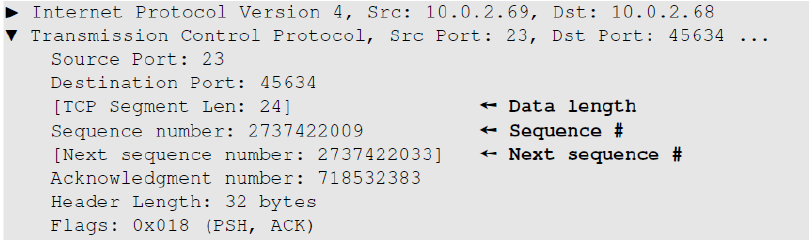
\includegraphics[width=1\linewidth]{images/codiceHijacking.png}
\end{figure}

\subsection{TCP hijacking attack ed esempio rispetto al codice}
Il TCP hijacking è un attacco in cui un attaccante prende il controllo di una sessione TCP già avviata tra due host, senza che uno dei due se ne accorga. L'attaccante invia pacchetti spoofati, fingendosi uno degli
endpoint, sfruttando il fatto che TCP si basa su numeri di sequenza e acknowledgment per mantenere la connessione affidabile. L'obiettivo dell'attacco è quello di iniettare dati o comandi nella sessione o interromperla/alterarla.

\noindent Nel nostro scenario ipotetico, l'attaccante intercetta un pacchetto proveniente dal server verso il client in una connessione Telnet. Anche se non conosce l'intero stato della sessione, dal pacchetto osservato può dedurre quale sarà il prossimo numero di sequenza atteso dal server.
A quel punto, può costruire un pacchetto contraffatto, con IP e porta del client e valori di sequenza e acknowledgment coerenti, inserendo nel payload un comando arbitrario da far eseguire alla shell remota. 
Poiché Telnet è un protocollo testuale non cifrato, il comando viene trasmesso come semplice testo ASCII e, se ben formato, sarà interpretato come input valido dal server.

\subsection{Codice}
Questo pacchetto è parte di una connessione Telnet attiva dal server verso il client. L'attaccante ha intercettato questo pacchetto e ora conosce i seguenti dati cruciali:
\begin{itemize}
    \item IP e porte della connessione
    \item Numero di sequenza attuale del server (2737422009)
    \item Numero di acknowledgment del server, che indica quale byte si aspetta dal client (718532383).
    \item La dimensione del payload (24 byte) che è la differenza tra sequence number e next sequence number.
\end{itemize}

\begin{center}
    \textbf{Qual è il pacchetto da da spedire per portare a termine l'attacco?}
\end{center}
\noindent L'attaccante vuole fingere di essere il client che invia dati al server. Per fare ciò, costruisce un pacchetto spoofato con questi campi:
\begin{itemize}
    \item \textbf{Src IP:} 10.0.2.68 (IP del client)
    \item \textbf{Dst IP:} 10.0.2.69 (IP del server)
    \item \textbf{Src Port:} 45634 (porta del client)
    \item \textbf{Dst Port:} 23 (porta standard per Telnet)
    \item \textbf{Sequence number:} 718532383 (numero di sequenza che il server si aspetta dal client)
    \item \textbf{Acknowledgment number:} 2737422033
    \item \textbf{Flags:} PSH,ACK
    \item \textbf{Payload:} ls\textbackslash n (per esempio)
\end{itemize}

\noindent \textit{Note dell'autrice:} 
\begin{itemize}
    \item per trovare Src e Dst IP letteralmente inverti i due indirizzi iniziali
    \item Src Port è quella che prima stava sotto la dicitura Destination Port
    \item il Sequence number è quello che prima si chimava acknowledgment number 
    \item l'acknowledgment number è il nezt sequence number
    \item le flags le copiamo
    \item Importante excursus sul payload: è necessario se vogliamo far eseguire al server un comando, va bene qualsiasi comando Telnet io ho mesos questo a caso
\end{itemize}

\begin{center}
    \textbf{Nel caso si voglia far eseguire un comando al server, come si può procedere?}
\end{center}
\noindent La risposta a sto point è chiaramente il payload!!

\noindent Per far sì che il server esegua un comando (es. in una sessione Telnet), è necessario
inserire nel pacchetto un payload contenente il comando, terminato da un carattere di newline (\textbackslash n), come avverrebbe nella digitazione manuale da parte dell'utente,
ricordandosi che il comando deve avere senso nel contesto della shell remota.






\section{Approcci alla scansione + FTP bounce scan}
\noindent La scansione all'interno di una rete viene eseguita per recuperare informazioni su determinati host o server, l'obiettivo principale è ottenere informazioni
sulle porta utilizzate (TCP/UDP), ciò quali porte sono aperte e in ascolto su determinati nodi, oltre che determinare quale sistema operativo è presente e se esistono sistemi di filtraggio o 
firewall in una determinata rete.

\noindent Lo scanning può essere attivo o passivo:
\begin{itemize}
    \item \textbf{Attivo:} si immette traffico nella rete per recuperare informazioni
    \item \textbf{Passivo:} si fa sniffing senza intervenire attivamente
\end{itemize}

\noindent Diversi approcci:
\begin{itemize}
    \item \textbf{Verticale:} host che fa scanning di più target 
    \item \textbf{Orizzontale:} molti host fanno scanning sullo stesso target 
    \item \textbf{Ibrido:} mix tra i due
\end{itemize}

\noindent Infine il target può essere \textbf{singolo}, cioè una macchina, o \textbf{multiplo}, cioè anche una porzione di rete (se non tutta).

\subsection{FTP bounce scan}
L'attacco FTP bounce scan è una tecnica utilizzata per eseguire una scansione delle porte (port scanning) di un host di destinazione indirettamente tramite un server FTP, è una delle tecniche più note di port scanning attraverso terze parti.

\noindent L'attaccante invia al server FTP un comando PORT utilizzando l'indirizzo IP della vittima tramite un pacchetto spoofato.
Se la porta del server è chiusa, quest'ultima risponderà con un pacchetto RST alla richiesta proveniente dal server FTP, mentre verrà eseguita una three-way handshake nel caso in cui la porta fosse aperta.


\subsection{Commentare praticamente il risultato della seguente scansione}

\begin{figure}[H]
    \centering
    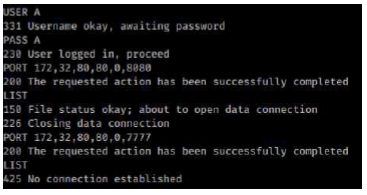
\includegraphics[width=1\linewidth]{images/scansione.png}
\end{figure}
L'attaccante, utilizzando il comando port, riesce a capire che la porta 8080 è aperta (e quindi in ascolto), dato che viene indicato che è possibile trasferire file, mentre la porta 7777 non lo è, dato che non è stata stabilita nessuna connessione.

\subsection{Due tecniche di scansione con TCP}
\subsubsection{TCP Connect Scan}
Questa tecnica tenta di stabilire una connessione TCP completa con la porta target inviando un pacchetto SYN, aspettando la risposta SYN-ACK e completando il handshake con un ACK.

\noindent Se la connessione si stabilisce, la porta è aperta.
Se riceve un pacchetto RST (reset), la porta è chiusa.

\noindent E' semplice da implementare ma rumoroso.

\subsubsection{SYN Scan (Half-open scan)}
Invia un pacchetto SYN al target, ma non completa il handshake. Se riceve un SYN-ACK, invia un pacchetto RST per interrompere la connessione prima che venga completata.

\noindent Se riceve un SYN-ACK la porta è aperta, se riceve RST allora è chiusa.

\noindent Più furiva della connect scan poichè non comporta connessione, ma può essere rilevata da firewall 


\section{Reset Attack}
Un TCP Reset Attack (attacco di reset TCP) è una tecnica usata per interrompere una connessione TCP esistente inviando un pacchetto TCP con il flag RST (Reset) attivo.
\begin{figure}[H]
    \centering
    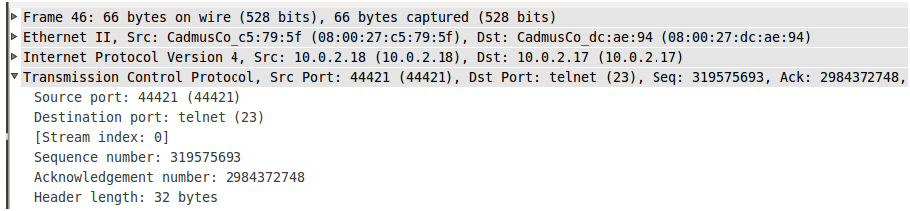
\includegraphics[width=1\linewidth]{images/reset.png}
\end{figure}
\noindent In una normale comunicazione TCP, il flag RST viene usato per indicare che qualcosa è andato storto e che la connessione deve essere chiusa immediatamente.
Un attaccante, intercettando o osservando una connessione TCP, invia un pacchetto con flag RST a uno o entrambi i lati della connessione.




\chapter{Attacchi}

\section{Problematiche di sicurezza del protocollo SSL}
\begin{itemize}
    \item le preferenze sulla cipher suite non sono autenticate
    \item usa MD5 come algoritmo hash per il MAC
    \item tutti i messaggi dell'hashake non sono protetti
    \item non supporta catene di certificazione o algoritmi non-RSA
\end{itemize}

E' inoltre possibile fare un man in the middle facendo ARP cache poisoning e posizionandosi come nodo
tra client e server in maniera trasparente

\section{Problematiche di sicurezza del protocollo ARP e discutere ARP poisoning attack}
Il protocollo di ARP va ad associare un indirizzo fisico (MAC) a un indirizzo logico (IP): ogni client possiede una tabella cache in cui vengono inserite le associazioni già attive. Se non fosse presente una voce, viene fatta una richiesta in broadcast a tutti i nodi della LAN (viene chiesto chi ha un certo indirizzo IP).
Questo genere di messaggi è vulnerabile ad attacchi di spoofing, in quanto si può impersonare un certo nodo della LAN e quindi eventualmente ricevere traffico che non sarebbe destinato all’attaccante.
La tipologia di attacco definita ARP poisoning attack consiste nel generare diversi pacchetti spoofati di ARP request in modo da andare a riempire la tabella di cache di informazioni non corrette causando disservizi e rallentamenti nelle comunicazioni tra le LAN.

\section{Descrivere in cosa consiste IP spoofing, e in dettaglio attacchi che fanno uso di tale tecnica}
IP spoofing è un tipo di attacco in cui un client malevolo modifica un pacchetto andando a inserire un altro indirizzo IP rispetto al prossimo, con lo scopo di ingannare una vittima e fare il man in the middle in una determinata comunicazione, oppure può causare un denial of service in quanto può interrompere una connessione o causarne il congestionamento inviando diversi pacchetti.
Esistono due tipologie di IP spoofing: non-blind, cioè che l'attaccante cerca di farsi passare per un host della sua stessa LAN, oppure blind, in cui l’attaccante cerca di farsi passare per un host di una qualsiasi sottorete.
Gli attacchi di IP spoofing cercano di predirre il sequence number del target per potersi frapporre nella comunicazione, dopodiché si cerca di instaurare un three-way handshake per recuperare informazioni o anche solo causare denial of service.


\section{Descrivere in dettaglio l'attacco basato su MAC flooding, conseguenze ed eventuali contromisure}
Il MAC flooding consiste nell'inviare ad uno switch pacchetti appositamente costruiti per riempire la CAM table (Content Addressable Memory table) che permette di associare rapidamente un indirizzo MAC alla porta a cui è collegato il terminale dello switch, con indirizzi MAC fittizi.
Le tabelle degli indirizzi MAC hanno dimensioni limitate. Il MAC flooding fa uso di questa limitazione per inviare allo switch un intero gruppo di indirizzi MAC di origine falsa in modo da saturare la tabella. Quando la tabella è satura lo switch entra in fail-open mode e si comporta come un hub, ovvero invia i pacchetti che riceve a tutti i nodi collegati allo switch






\chapter{Scanning}
\section{tecnica IDLE scan illustrando con un esempio le risposte in caso di porta chiusa, aperta o filtrata}
Nel IDLE SCAN abbiamo un \textbf{attaccante}, una \textbf{vittima} e uno \textbf{zombie}, vale a dire un terzo attore che verrà sfruttato dall'attaccante per colpire la vittima indirettamente
e capire se una determinata porta è aperta, oppure no, utilizzando pacchetti TCP.

\noindent L'attaccante manda un pacchetto TCP di tipo SYN\textbackslash ACK allo zombie. Quest'ultimo non si aspetta questo messaggio, perciò risponde con un pacchetto RST e un IPID, vale a dire l'identificativo del frame (es. 12345).

\noindent L'attaccante invia un pacchetto SYN (con la porta da scansionare) spoofato, utilizzando come mittente l'indirizzo IP dello zombie, alla vittima: in questo caso, se la porta è in ascolto, la vittima risponderà 
allo zombie con un pacchetto SYN\textbackslash ACK e un IPID incrementato (es. 12346), a cui lo zombie risponde con un pacchetto RST, in quanto non si aspetta questo genere di comunicazione.

\noindent Infine l'attaccante invia un altro pacchetto di SYN\textbackslash ACK allo zombie, che gli risponde con un RST e un IPID incrementato (es. 12347): confrontando i valori di IPID, l'attaccante capisce che la porta è aperta.

\noindent Se invece la porta fosse chiusa o filtrata, il valore di IPID sarebbe stato incrementato una sola volta, in quanto l'attaccante risponderebbe rispettivamente con un RST o non risponderebbe affatto al pacchetto 
spoofato inviato dall'attaccante, fingendosi lo zombie. 
Con il secondo SYN\textbackslash ACK allo zombie, ci sarebbe quindi solo questo incremento di IPID.

\subsection{contesto della porta 23 della vittima sapendo che l'ultima risposta ottenuta dallo zombie ha id=42380}
L'attaccante vuole capire lo stato della porta TCP 23 del target/vittima usando lo zombie
quindi invia un pacchetto SYN al target con IP sorgente spoofato dello zombie.

\section{ Descrivere sinteticamente i metodi di scansione stealth}
\noindent I meccanismi di scansione stealth sono \textbf{tecniche usate per identificare porte aperte su un sistema senza suscitare allarmi o lasciare tracce evidenti nei log}, cercando di evitare il rilevamento da parte di firewall, IDS (Intrusion Detection System) o sistemi di logging.

\noindent Principi base delle scansioni stealth:
\begin{itemize}
    \item \textbf{Evitare handshake completo:} invece di completare la connessione TCP (che è facilmente loggabile), si inviano pacchetti parziali o particolari per sondare la risposta
    \item \textbf{Minimizzare i pacchetti inviati:} meno traffico significa meno probabilità di essere rilevati
    \item \textbf{Usare pacchetti con flag TCP “particolari”:} per confondere filtri e firewall
\end{itemize}

\section{Differenza tra le tecniche scan stealth e non stealth}
\noindent \textbf{\textit{NON} STEALTH:}
\begin{itemize}
    \item Completano il normale handshake TCP a 3 vie, aprendo una connessione completa con la porta target
    \item Vengono registrate nei log del sistema target 
    \item Facili da rilevare e bloccare, poichè utilizzano pacchetti standard senza trucchi particolari
\end{itemize}

\noindent \textbf{STEALTH:}
\begin{itemize}
    \item Non completano il handshake TCP o inviano pacchetti con flag TCP particolari per evitare di stabilire una connessione completa
    \item Invia meno pacchetti o pacchetti meno “comuni” per confondere firewall e filtri
    \item Ridotta probabilità di essere registrati nei log o rilevati da IDS
\end{itemize}



\chapter{Network Scanning}
\section{Riconoscere e commentare il tipo di scan evidenziato in figura e aggiungere il caso mancante (porta chiusa/aperta)}
\begin{figure}[H]
    \centering
    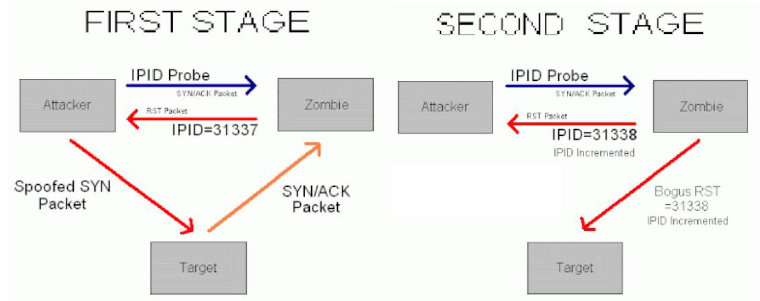
\includegraphics[width=1\linewidth]{images/scanEvidenziato.png}
\end{figure}

\noindent Il tipo di attacco è conosciuto come IDLE scan in cui viene utilizzato 
un client intermedio come \textbf{zombie} per rendere complicata risalire all'attaccante. 
La sorgente manda un SYN/ACK allo zombie e aspetta un RST come risposta con IPID. 
Successivamente l'attaccante invia un pacchetto SYN spoofato con IP sorgente del client zombie verso 
la vittima con la porta che vuole scansionare. 
Se la porta è aperta, la vittima risponderà con un SYN/ACK allo zombie. Quest'ultimo non si aspetta un SYN/ACK e risponde 
perciò con un messaggio RST e con un IPID+1. 

\noindent Infine l'attaccante manda nuovamente un pacchetto SYN/ACK al client zombie e, se IPID è aumentato, allora la porta è aperta.

\noindent Manca il caso in cui la porta è chiusa o filtrata: in questo caso IPID non viene aumentato; quindi, l'attaccante capisce che non c'è traffico su quella specifica porta.

\section{Descrivere quali sono le condizioni rilevabili di una porta come risultato di uno scanning e cosa indicano ad un potenziale avversario e 
per ciascuno stato fare un esempio di un tipo di scan che produca quel tipo di stato}

\subsection{condizioni rilevabili}
Una porta può essere:
\begin{itemize}
    \item \textbf{aperta:} quindi un servizio è in ascolto su di essa
    \item \textbf{chiusa:} quindi non c'è nulla in ascolto su di essa 
    \item \textbf{filtrata:} cioè che è presente un firewall che permette l'accesso solo a determinate sorgenti (in quest'ultimo caso non è possibile definire se è aperta o chiusa)
\end{itemize} 

\subsection{esempio per tipo:}
Per testare lo stato di una porta, si può fare un TCP SYN scan che consiste nell'inviare un pacchetto TCP di tipo SYN + la porta da scansionare,
simulando un three-way handshake: se la porta restituisce un pacchetto SYN/ACK, 
allora la porta è aperta, mentre se restituisco un RST, allora è chiusa. Nel caso di una porta filtrata, il comportamento dipende dal firewall.


\section{obiettivi, natura degli approcci al port scanning}
Guardare 5.4
\subsection{risultati possibili per la scansione di una porta}
Una porta può essere in tre stati: aperta, nel senso che c'è un protocollo in ascolto su di essa, pronto per far partire una comunicazione TCP.
chiusa, vale a dire che non è presente nessun protocollo in ascolto e infine filtrata, cioè che è presente un firewall che lascia passare del traffico
su una porta solo a determinate condizioni, come per esempio la provenienza da determinati indirizzi.
In quest'ultimo caso non è possibile capire se un determinato protocollo è in ascolto o meno.

\subsection{Descrivere in dettaglio un approccio allo scan}
IDLE, guardare 7.1




\chapter{Firewall e NIDS}
\section{Descrivere come funziona un firewall stateful}
Uno stateful firewall analizza ogni pacchetto che lo attraversa singolarmente e in più tiene traccia delle connessioni e del loro stato, grazie 
a una tabella dello stato interna al firewall nella quale ogni connessione TCP e UDP viene rappresentata da due coppie formate da indirizzo IP e porta, 
una per ciascun endpoint della comunicazione.

\section{Cosa è un IDS? Descrivere una possibile integrazione tra IDS e firewall}
L'IDS è un sistema di monitoraggio utilizzato per identificare accessi non autorizzati a pc o reti locali. Ha tecniche e metodi realizzati per rilevare pacchetti 
dati sospetti a livello di rete, trasporto e applicazione. 

\noindent Un IDS non può bloccare o filtrare i pacchetti in ingresso ed in uscita, né può modificarli.

\noindent Una possibile integrazione tra firewall e IDS:

\noindent Un IPS (intrusion prevention system) invece è comunemente considerato l’accoppiata tra firewall e IDS, cioè si parla di una tecnologia, che cerca di bloccare attacchi alle fasi 
preliminari, facendo analisi predittiva sulla base di informazioni precedenti ricevute.

\section{Cosa si intende per stateful firewall? Che differenza esiste con un firewall stateless?}
\subsection{Stateful firewall}
I firewall stateful sono in grado di riconoscere le connessioni e le trasmissioni e, ispezionandole, sono in grado di decidere cosa fare in base a molteplici parametri.
\noindent Del traffico mantengono un log storico, con i dettagli relativi (indirizzi di origine e destinazione, numeri di porta, sequenze TCP, ecc.) e con questo sono in gradi di 
aprire o chiudere dinamicamente delle porte per consentire o bloccare il traffico.

\subsection{Stateless firewall}
I firewall stateless invece bloccano o consentono una comunicazione soltanto sulla base delle caratteristiche di quest'ultima. 

\noindent In pratica i pacchetti sono bloccati in base a delle regole statiche (ad es. l'indirizzo sorgente o quello di destinazione, la porta utilizzata) e di ciò non viene tenuta memoria.

\section{Come funziona un IDS e quali sono le differenze rispetto ad un IPS}
\subsection{IDS}
Un IDS (intrusion detection system) è un sistema di monitoraggio utilizzato per identificare dei comportamenti malevoli, rilevando attacchi o altre violazioni alla sicurezza e 
fornendo informazioni su intrusioni avvenute, grazie all'uso di sonde posizionate sugli host, oppure in certi punti della rete.

\noindent Ci sono due tipologie di IDS: \textbf{passivi}, che fanno un controllo di firme, e \textbf{attivi}, che apprendono i dati del sistema e “imparano” dall’analisi statistica del funzionamento del sistema.

\subsubsection{Dove andrebbe posizionato in una rete che abbia due accessi ad internet}
In una rete con due accessi a Internet, un IDS va posizionato in un punto centrale dove converga il traffico proveniente da entrambi i collegamenti, dietro i firewall o router, ma prima della rete interna. Questo permette di monitorare tutto il traffico in ingresso e in uscita, indipendentemente da quale connessione venga utilizzata, garantendo una rilevazione completa delle eventuali minacce. 
Se i due accessi sono completamente separati, può essere necessario un IDS per ciascun punto o un sistema che raccolga il traffico da entrambi.

\subsection{IPS}
Un IPS (intrusion prevention system) invece è comunemente considerato l'accoppiata tra firewall e IDS, cioè si parla di una tecnologia, 
che cerca di bloccare attacchi alle fasi preliminari, facendo analisi predittiva sulla base di informazioni precedenti ricevute.

\noindent La prevenzione è intesa come velocizzazione dei tempi di risposta una volta che si individua un attacco, il problema relativo a questa tecnologia è il rischio di prendere decisioni sbagliate in automatico o il bloccaggio
di traffico innocuo
\subsubsection{Come realizzare IPS:}
Per esempio si può utilizzare Snort (IDS open source molto noto e testato) in modalità inline mode, che riceve i pacchetti direttamente da iptable e collabora per bloccare il
traffico sospetto.


\section{Illustrare le differenze tra application-level gateway e circuit-level gateway}
\subsection{application-level gateway}
Un application-level gateway è composto da una serie di proxy che esaminano il contenuto dei pacchetti a \textbf{livello applicativo}, fornendo un livello di sicurezza maggiore (es. contro attacchi di buffer overflow): 
posizionandosi tra client e server, impedisce la comunicazione diretta e può offrire anche servizi di load balancing del traffico.

\subsection{circuit-level gateway}
Un circuit-level gateway invece è un circuito tra client e server a  \textbf{livello di trasporto} (non applicativo), perciò non fa inspection del traffico che gli passa, ma si occupa solo di tenere traccia delle comunicazioni sul circuito. 
Anch'esso spezza il modello client\textbackslash server, facendo da tramite, ma a tutti gli effetti non fornisce sicurezza lato applicativo.

\section{Cosa si intende per deep packet inspection? Quali funzioni addizionali si trovano
generalmente integrate in firewall di questo tipo? Come si applicano a scenari di encrypted threats?}
\subsection{deep packet inspection}
La deep packet inspection è una tecnica di packet filtering che va a controllare il contenuto dei pacchetti in transito in maniera approfondita, per identificare codice malevolo.
A differenza dei metodi tradizionali che si limitano a ispezionare intestazioni (header) di pacchetti IP, la DPI analizza il contenuto completo dei pacchetti, compreso il payload, per identificare protocolli, applicazioni, comportamenti sospetti o specifici pattern di dati.

\subsection{funzioni addizionali}
\begin{itemize}
    \item \textbf{Application Control (Controllo delle applicazioni):} Permette di identificare e controllare il traffico in base all'applicazione, non solo in base alla porta o al protocollo.
    \item \textbf{Intrusion Detection and Prevention (IDS/IPS):} Identifica comportamenti malevoli nel traffico di rete (es. exploit noti, attacchi buffer overflow).
    \item \textbf{Data Loss Prevention (DLP):}Identifica tentativi di esfiltrazione di dati sensibili, come numeri di carte di credito, codici fiscali, documenti riservati.
\end{itemize}

\subsection{scenari di encrypted threats}
In scenari di encrypted threats, la deep packet inspection può mettersi in mezzo a una comunicazione criptata in quanto è possibile abilitare la possibilità di far verificare un traffico cryptato per poter capire se è presente un man in the 
middle che sta sfruttando un canale cifrato per attaccare una rete: la procedura consiste nell'inviare i pacchetti su un server in cloud che fa analisi e mi dice se la connessione è “pulita” o se sono presenti minacce. 

\section{Principi inderogabili dei firewall}
Sono 3:
\begin{itemize}
    \item un fireall deve essere l'unico punto di contatto della rete interna con quella esterna
    \item solo il traffico autorizzato può attraversare il firewall
    \item il firewall deve essere esso stesso un sistema altamente sicuro
\end{itemize}

\section{proxy firewall}
Mediano connessioni applicative e gestiscono aspetti di sicurezza.
un proxy firewall è generalmente composto da una serie di proxy che esaminano il contenuto dei
pacchetti a livello applicativo.

\noindent Nell'interazione con le applicazioni, usare un approccio con ALG richiede uno specifico proxy per
ogni applicazione il che comporta un ritardo nel supporto, maggiore consumo di risorse e basse prestazioni.
Ha però il vantaggio di rompere il modello client/server tipico, cosa che da maggiore protezione ai
server.

\noindent In breve i vantaggi sono:
\begin{itemize}
    \item non permette connessioni dirette tra interno e esterno
    \item supporta l'autenticazione
    \item analizza i comandi a livello applicativo
    \item mantiene log del traffico e delle attività svolte
    \item analisi migliore del traffico applicativo rispetto ad un firewall stateful
\end{itemize}

\subsection{Configurazione reverse proxy}
Un reverse proxy è utilizzato per garantire l'accesso degli utenti esterni a risorse interne in modo sicuro e controllato. Si interpone tra i client e i server interni, inoltrando le richieste e nascondendo l'infrastruttura reale. 
Questo permette di proteggere i sistemi interni, applicare regole di accesso centralizzate e gestire le comunicazioni in modo efficiente e sicuro.

\section{Come funziona una honey pot? A cosa serve e come la potrei realizare?}
Una honeypot è un sistema di sicurezza informatica progettato per attirare, rilevare, deviare o studiare attacchi informatici. Si tratta di un sistema fittizio che simula 
una risorsa vulnerabile, come un server, un'applicazione o una rete, con l'obiettivo di ingannare gli attaccanti facendoli credere di aver trovato un bersaglio utile.
viene realizzata una sorta di rete ”finta” (la honey pot) per attirare gli attacchi poichè quando un attaccante
vuole entrare, di norma usa falle note, quindi si realizza una rete ad hoc per osservare come gli attacchi
vengano perpetrati. per questa ragione, si realizza una DMZ (generalmente `e una sandbox) proprio a questo
scopo.
non sono molto usate, ma vengono quasi sempre usate dai provider di sistemi di sicurezza per osservare
le vulnerabilità in un sistema e fare le patch occorrente. nell'honey pot di norma si mettono moltissimi
sensori IDS per misurare tutto quello che avviene.

\section{Descrivere come funziona iptables in dettaglio}
E' uno strumento della suite netfilter di Linux usato per filtrare pacchetti di rete, NAT, forwarding e controllo del traffico. È ampiamente usato per creare firewall su sistemi Linux.
E' organizzato in:
\begin{itemize}
    \item \textbf{Tabelle:} Ogni tabella contiene catene (chains) che a loro volta contengono regole.
    \item \textbf{Catene:} Ogni tabella contiene catene predefinite (built-in) e personalizzate.
    \item \textbf{Regole:} Ogni catena contiene una lista di regole che specificano:
    \begin{itemize}
        \item \textit{Condizioni: }cosa deve essere vero per applicare la regola
        \item \textit{Azioni (target):} cosa fare se le condizioni corrispondono
    \end{itemize}
\end{itemize}

\section{FTP Bounce Attack, dire di cosa si tratta e quale
tipologia di firewall potrebbe bloccarlo e come}
L'FTP Bounce Attack è un attacco che sfrutta una caratteristica del protocollo FTP in modalità passiva (PORT command) 
per rimbalzare connessioni attraverso un server FTP verso altri host o porte.

\noindent Questo tipo di attacco è risolvibile con uno stateful firewall. un FTP proxy potrebbe riconscere un uso
imporprio del protocollo e terminare la connessione.
Nella pratica il problema è stato risolto con aggiornamenti degli FTP server

\section{Cosa è Snort e cosa permette di realizzare? Fare degli esempi di cosa si può ottenere}
Snort è un IDS open source molto noto e testato, è in grado di funzionare sia in modalità sniffer (osserva il traffico e logga) sia in modalità IDS.

\noindent Ha quattro modalità di utilizzo previste:
\begin{itemize}
    \item \textbf{sniffer mode:} legge i pacchetti dalla rete e li visualizza come un flusso continuo
    \item \textbf{packet logger mode:} logga i pacchetti salvandoli sul disco 
    \item \textbf{network intrusion detection system mode (funziona da NIDS):} utilizza regole snort-based per
individuare pattern di traffico sospetti
    \item \textbf{inline mode (funziona da IPS):} riceve i pacchetti direttamente da iptable e collabora per bloccare il
traffico sospetto.
\end{itemize}


\section{Cooperazione tra firewall e IPS}
Un firewall e un IPS (Intrusion Prevention System) sono entrambi dispositivi di sicurezza di rete, ma con funzioni complementari.
\begin{itemize}
    \item \textbf{Firewall:} Filtra il traffico in base a indirizzi IP, porte, protocolli, regole statiche
    \item \textbf{IPS:} Analizza il contenuto del traffico in profondità (payload), rileva attacchi, blocca minacce conosciute
\end{itemize}

\noindent Nella pratica l'IPS controlla il traffico permesso dal firewall ispezionando i pacchetti più ne dettaglio, cercando firme di attacchi noti e comportamenti anomali.

\subsubsection{Esempio pratico:}
L'utilizzo di entrambi potrebbe essere utile tipo nel caso di attacco SQL injection 



\section{Assumendo un firewall posizionato su un router, devono essere filtrati i traffici in
ingresso al firewall stesso o solo quelli che devono essere "forwarded"? Spiegare le
motivazioni constestualizzando lo scenario}
Quando un firewall è posizionato su un router, è fondamentale filtrare sia il traffico destinato al router stesso (INPUT) sia quello che deve essere inoltrato verso altre reti (FORWARD). 
Questo perché il router non è solo un punto di passaggio del traffico, ma anche un dispositivo esposto e potenzialmente attaccabile. Se non si filtrano le connessioni in ingresso dirette al router (come SSH, ping o interfacce web), un attaccante potrebbe comprometterne il controllo. 
Allo stesso tempo, filtrare solo il traffico inoltrato non protegge l'infrastruttura di rete in modo completo. Per garantire una sicurezza efficace, quindi, bisogna gestire entrambe le tipologie di traffico con regole di firewall adeguate, riducendo la superficie di attacco e controllando l'accesso tra le varie zone della rete.


\section{Descrivi tutti i tipi di firewall che conosci associando I diversi livelli ISO/OSI che sono in grado di analizzare}
\begin{itemize}
    \item \textbf{Firewall di tipo stateless:} forniscono packet filtering di tipo stateless, quindi un semplice controllo dei pacchetti in transito, basandosi su alcune regole preimpostate, principalmente legate a indirizzi di sorgente e destinazione (livello 3 ISO/OSI – Network).
    \item \textbf{Firewall di tipo stateful:} forniscono packet filtering di tipo stateful, in cui vengono analizzate più informazioni del pacchetto, comprese le porte utilizzate, i protocolli e viene tenuta traccia tramite log delle azioni. Inoltre si ricordano se una sessione TCP era attiva, così da far passare i pacchetti successivi (livello 4 ISO/OSI – Transport).
    \item \textbf{Application Gateway:} esaminano il contenuto dei pacchetti a livello applicativo, fornendo un livello di sicurezza maggiore (livello 7 – ISO/OSI – Application).
\end{itemize}


\section{Quali sistemi firewall riescono a controllare il traffico applicativo? Come funzionano?}
Un application-level gateway è composto da una serie di proxy che esaminano il contenuto dei pacchetti a livello applicativo, fornendo un livello di sicurezza maggiore (es. contro attacchi di buffer overflow): posizionandosi tra client e server, impedisce la comunicazione diretta e può offrire anche servizi di load balancing del traffico.
Se un firewall è un IDS (intrusion detection system) vengono utilizzati insieme, si può ottenere una tecnologia chiamata IPS (intrusion prevention system), che va a fare attività predittiva sulla base a informazioni ricevute in precedenza che permettono di bloccare certi attacchi sul nascere.



\end{document} 